\section{Wymagania techniczne}

\subsection{Wstępna specyfikacja sprzętu i oprogramowania podstawowego}
\begin{enumerate}
	\item System w wersji podstawowej będzie składał się z 2 serwerów. Każdy z serwerów będzie posiadał zainstalowany system Linux.
	\begin{itemize}
		\item serwer przechowywujący backendową część aplikacji, serwer webowy udostępniający usługę, oraz aplikację frontendową
		\item serwer przechowywujący bazę danych
	\end{itemize}
	
	\item Ze strony klienckiej wykorzystywana jest jedynie przeglądarka
	\item Komunikacja między serwerami oraz urządzeniami klientów jest zapewniona przez rounter sieci lokalnej z brakiem możliwości dostępu z zewnętrznej sieci
	\item Opcjonalnie możliwe jest użycie aplikacji przez skorzystanie z uslugi VPN uruchomionej na dodatkowym serwerze dostępowym
\end{enumerate}

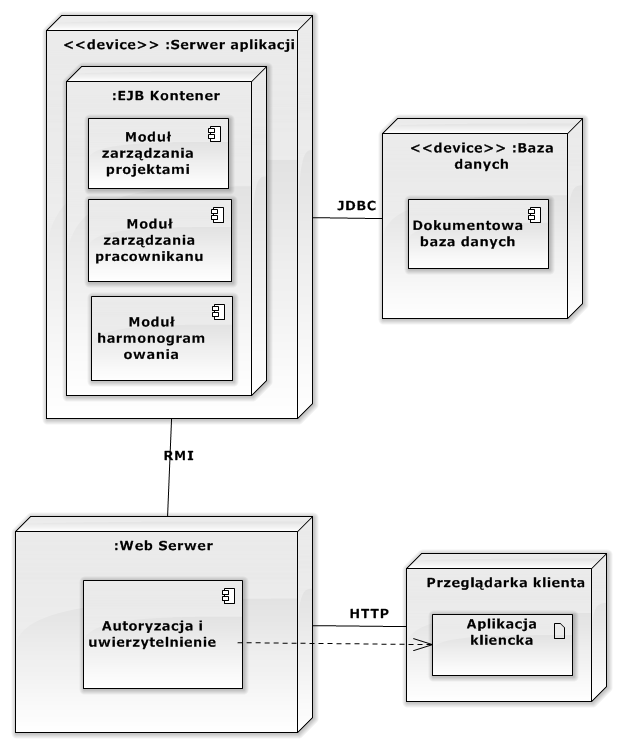
\includegraphics{deployment/Deploymentdiagram1}

\subsection{Specyfikacja technologii realizacji oprogramowania systemu}
\begin{enumerate}
	\item Aplikacja zostanie zrealizowana za pomocą technologii Java EE
	\item System bazy danych będzie zrealizowany jako baza NoSQL - w implementacji dokumentowej bazy danych MangoDB. Rozwiązanie to umżliwia szybki dostęp do ustrukturyzowanych danych.
	\item Aplikacja kliencka musi działać i być wyświetlana poprawnie pod przeglądarkami Chrome, Opera i Firefox, oraz Internet Explorer w wersji 8 i wyżej
	\item Frontend aplikacji klienckiej zostanie zrealizowany w technologii HTML5, CSS 3.00 oraz JavaScript
Jako serwer webowy zostanie użyty GlassFish Server
\end{enumerate}

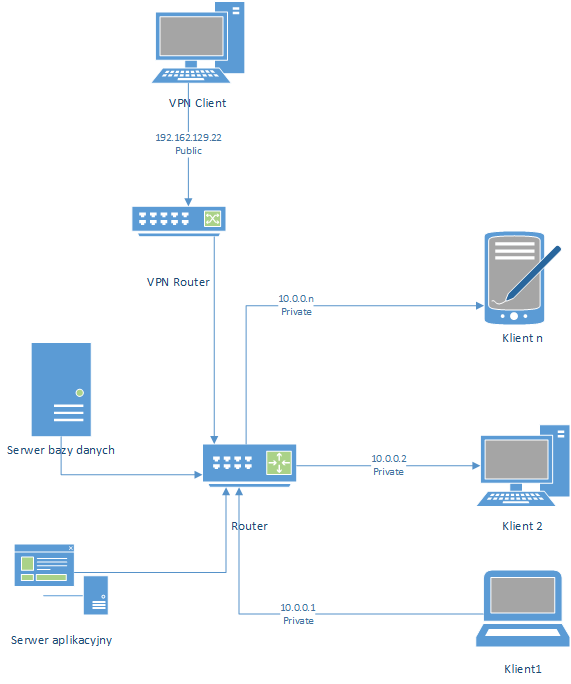
\includegraphics{deployment/siec}